%!TEX root = ../../Compte-rendu.tex
\subsection{Résultats}

\begin{figure}[H]
	\begin{center}
		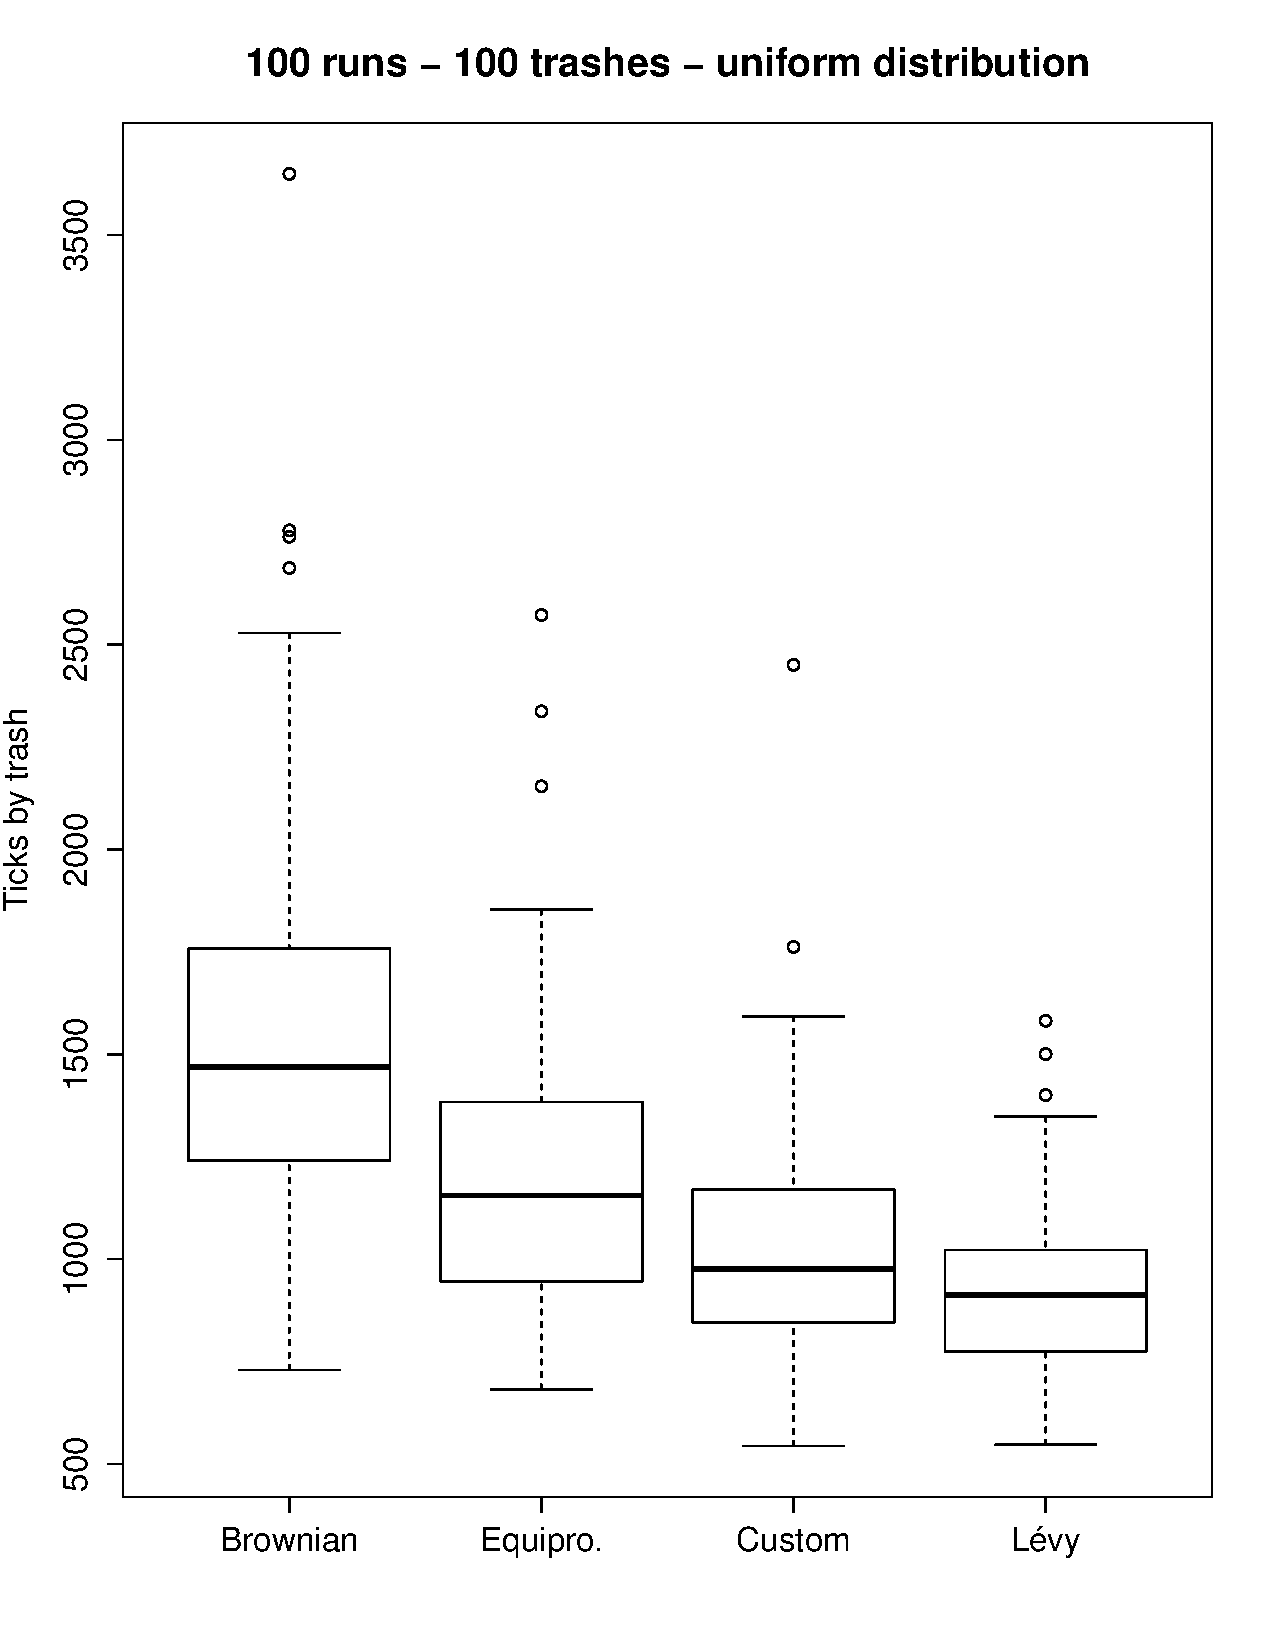
\includegraphics[height=8cm]{diagrams/100TrRnd_all.pdf}
		\caption{}
		\label{fig:}
	\end{center}
\end{figure}


\begin{figure}[H]
	\begin{center}
		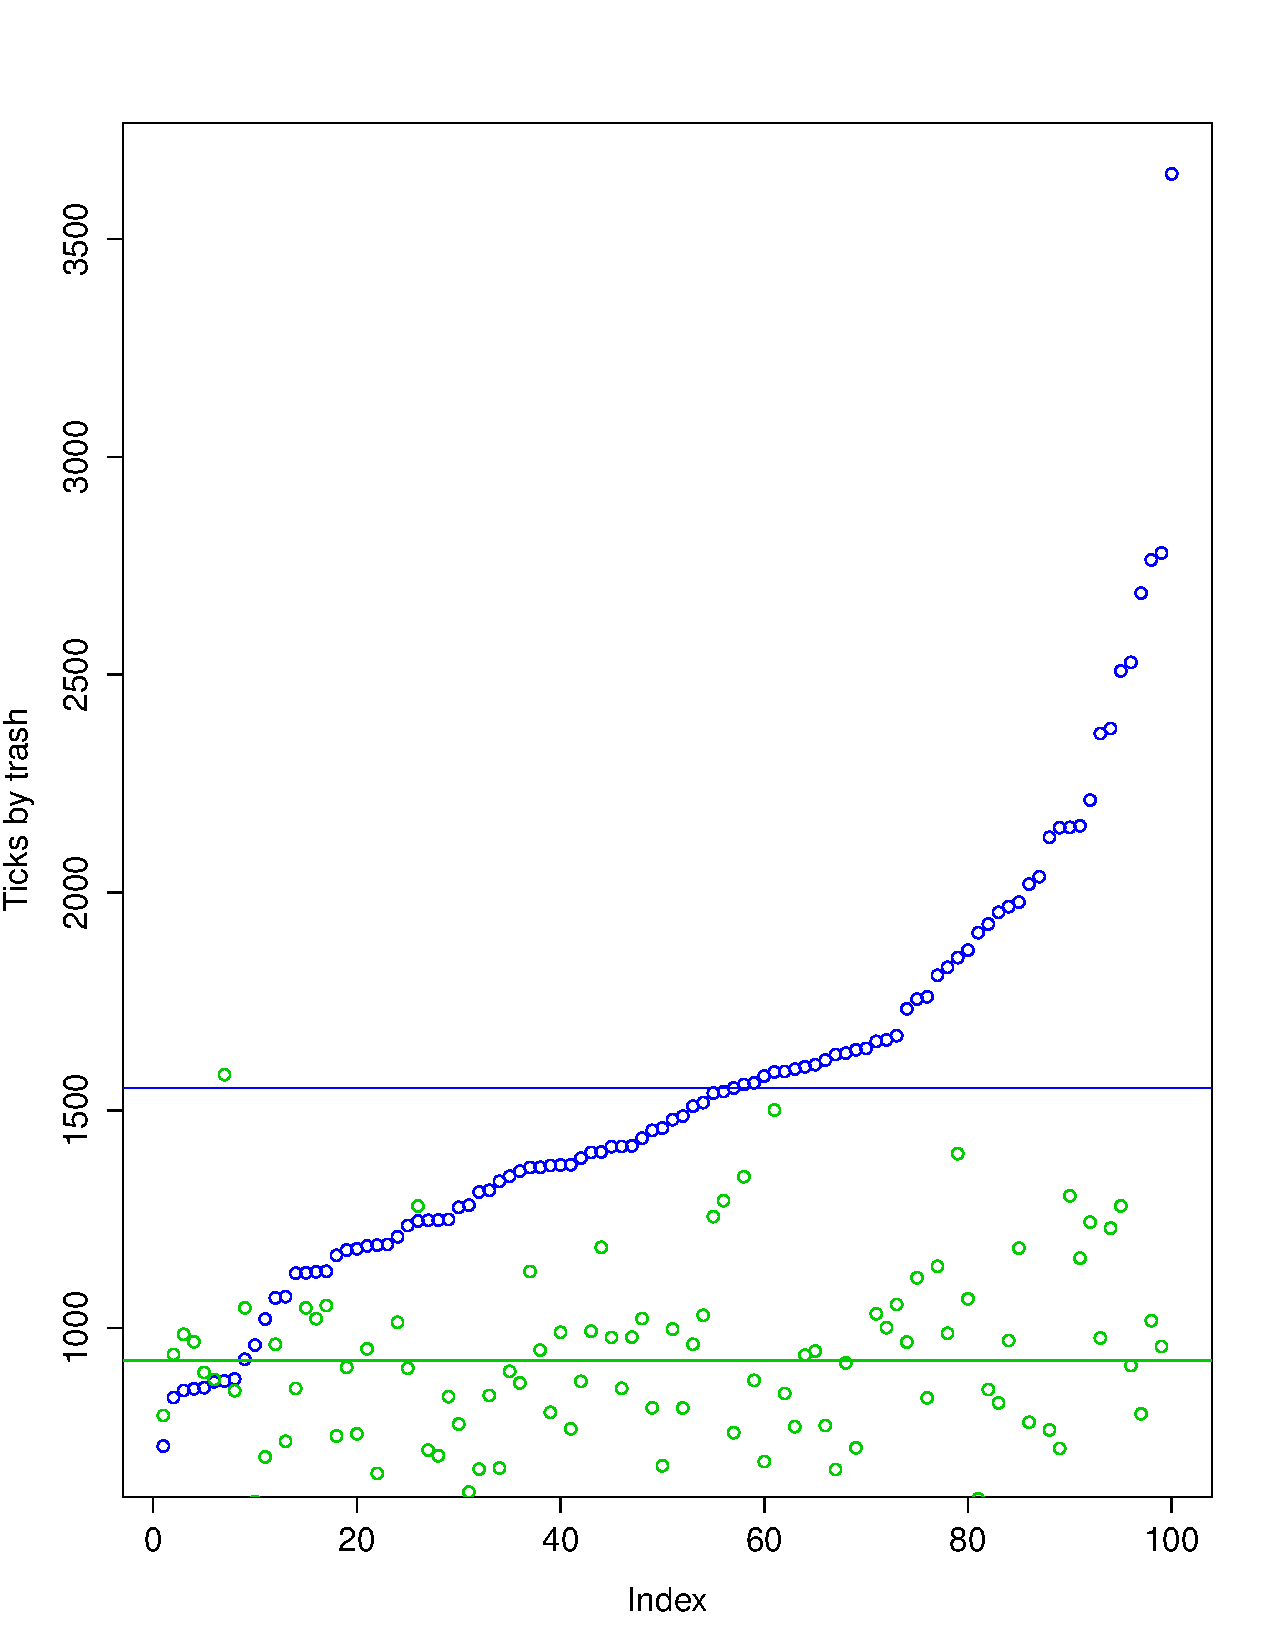
\includegraphics[height=8cm]{diagrams/100TrRnd_brow_levis.pdf}
		\caption{}
		\label{fig:}
	\end{center}
\end{figure}

> mean(dataToDisplay$Brownian)
[1] 1550.538
> mean(dataToDisplay$Equiprobable)
[1] 1197.424
> mean(dataToDisplay$Custom)
[1] 1035.69
> mean(dataToDisplay$Lévis)
[1] 925.1185